\subsection{Wormlike chain model(类蠕虫状链模型)}

连续高斯链是描述柔性聚合物链构型统计量的一种非常方便的理想链模型。然而,生物系统中遇到的许多大分子和某些合成聚合物,如液晶聚合物(LCPs)和共轭聚合物,都采用了比随机线圈(random coils)更接近刚性棒的构型态。为了描述这种被称为半柔性的系统,一个更合适的连续链模型是Kratky-Porod模型(Kratky和Porod,1949;Saito等人,1967)。这种模型也通常被称为类蠕虫状链。

我们可以想到,连续高斯链模型包含了局部链拉伸的调和能量损失,而不包含对链弯曲的能量损失。相反,类虫状链的每个微分段都被限制为不可扩展的,但是局部弯曲有一个调和能量损失。不扩展约束意味着聚合物的总轮廓长度$L_c$对所有所有链构型来说是常数。类虫状链的构型再次用空间曲线$\mathrm{r}(s)$描述,其中$s\in [0,L_c]$是描述聚合物主链弧长的参数。向量$\mathrm{u}(s)=d\mathrm{r}(s)/ds$是轮廓位置$s$处链的切线向量,并被约束为单位向量,$|\mathrm{u}(s)| =1$。向量$d\mathrm{u}(s)/ds=d^2\mathrm{r}(s)/ds^2$的大小可以类似地解释为聚合物在轮廓位置$s$处的局部曲率。通过沿着链状轮廓对调和曲率分布的求和,得到了类蠕虫链弯曲能的表达式:\\
\begin{equation}
	U_0[\mathrm{u}]=\frac{\lambda k_B T}{2}\int_{0}^{L_c}ds|\frac{d\mathrm{u}(s)}{ds}|^2 \label{类蠕虫链弯曲能表达式}
\end{equation}
微观参数$\lambda$具有单位长度,其物理意义将在短期内讨论。方程(\ref{类蠕虫链弯曲能表达式})中使用的表示法意味着弯曲势$U_0$是$\mathrm{u}(s)$的一个函数。然而,由于$\mathrm{u}(s)=d\mathrm{r}(s)/ds$,它也可以看作是聚合物形状$\mathrm{r}(s)$的函数。在将类蠕虫链的配分函数写成路径积分时,可以方便地将此约束和$|\mathrm{u}(s)|=1$的约束显式化:\\
\begin{equation}
	Z_0=\int \mathcal{D} \mathrm{r}\ \exp (-\beta U_0[\mathrm{u}])\prod_s\left[\delta\left(\mathrm{u}(s)-\frac{d\mathrm{r}(s)}{ds}\right)\delta(|\mathrm{u}(s)|-1)\right]\label{类蠕虫链的配分函数加约束}
\end{equation}
因此,在计算类蠕虫链配分函数时,我们要在所有链路径$\mathrm{r}(s)$上求和,与$\mathrm{u}(s)$是所有轮廓位置$s$上的单位切线向量一致。\\

由于这些约束条件,方程(\ref{类蠕虫链的配分函数加约束})很难直接作为路径积分来处理。相反,我们再次转向我们的随机过程类比,并考虑一个\textbf{约化分布函数}$p_0(\mathrm{r},\mathrm{u},s)$。这个量被定义为轮廓长度s的类蠕虫链的末端位于位置$\mathrm{r}$且末端段的切线向量为$\mathrm{u}$的概率密度。我们假定一种归一化,使得$\int d\mathrm{r}\int d\mathrm{u} \ p_0(\mathrm{r},\mathrm{u},s)=1$,其中$\mathrm{u}$上的积分表示单位球面上的积分。考虑链端位置和指向的分布函数的动机是,在建立半柔性聚合物模型时,我们通常希望考虑链段间的各向异性相互作用,例如LCPs中的向列相互作用。如第四章将展示的,这种相互作用的描述需要同时提供关于片段方向和位置的信息。

关于概率密度$p_0(\mathrm{r},\mathrm{u},s)$的Chapman-Kolmogorov方程的发展与惯性部分的布朗运动理论密切相关(Chandrasekhar,1943)。特别是,我们可以调用方程(\ref{类蠕虫链的配分函数加约束})的Markov性质,有\\
\begin{equation}
\begin{aligned}
	p_0(\mathrm{r},\mathrm{u},s+\Delta s)=\int d(\Delta \mathrm{r})\int d(\Delta \mathrm{u})\ &\Psi\  (\Delta \mathrm{r},\Delta \mathrm{u};\mathrm{r}-\Delta \mathrm{r},\mathrm{u}-\Delta \mathrm{u})\\ &\times p_0(\mathrm{r}-\Delta \mathrm{r},\mathrm{u}-\Delta \mathrm{u},s)\label{概率密度的Chapman-Kolmogorov方程}
\end{aligned}
\end{equation}
其中,$\Delta\mathrm{u}$表示切线向量的差分位移,$\Delta \mathrm{r}$表示与添加长度$\Delta \mathrm{s}$的链段相关联的末端位置的差分位移。函数$\Psi(\Delta \mathrm{r},\Delta \mathrm{u};\mathrm{r},\mathrm{u})$描述了添加的链段有位置和指向位移$\Delta \mathrm{r}$和$\Delta \mathrm{u}$的条件跃迁概率,从位置$\mathrm{r}$和指向$\mathrm{u}$开始.该跃迁概率被规范化,使得$\int d(\Delta \mathrm{r})\int d(\Delta \mathrm{u})\ \Psi=1$。在上面的积分中,应该注意到$\Delta\mathrm{u}$被限制为旋转,因此$\mathrm{u}$和$\mathrm{u}-\Delta \mathrm{u}$反映了单位球面上的附近点。从关系\\
\begin{equation}
\Delta \mathrm{r} = \int_{s}^{s+\Delta s}ds\ \mathrm{u}(s)
= \mathrm{u}\Delta s +O(\Delta s ^2)
\end{equation}
我们发现,过程(\ref{概率密度的Chapman-Kolmogorov方程})的随机性质,在$\Delta s$上是一阶的,仅限于变量$\Delta \mathrm{u}$。因此,我们可以将$\Delta \mathrm{r}$看作是确定性的,并降低跃迁概率为形式\\
\begin{equation}
	\Psi(\Delta \mathrm{r} ,\Delta \mathrm{u} ;\mathrm{r}, \mathbf{u})=\Phi(\Delta \mathrm{u};\mathrm{r},\mathrm{u})\ \delta(\Delta \mathrm{r}-\mathrm{u}\Delta s)\label{跃迁概率}
\end{equation}
其中,$\Phi(\Delta \mathrm{u};\mathrm{r},\mathrm{u})$是单位球面上与轮廓步长$\Delta s$相关的指向位移$\Delta \mathrm{u}$的归一化跃迁概率。通过$\mathrm{r}\longrightarrow \mathrm{r}+\mathrm{u}\Delta s$将方程(\ref{跃迁概率})代入方程(\ref{概率密度的Chapman-Kolmogorov方程}),得到简化的Chapman-Komogorov方程\\
\begin{equation}
	p_0(\mathrm{r}+\mathrm{u}\Delta s,\mathrm{u},s+\Delta s)=\int d (\Delta u)\ \Phi(\Delta \mathrm{u} ;\mathrm{r},\mathrm{u}-\Delta \mathrm{u})\ p_0(\mathrm{r},\mathrm{u}-\Delta \mathrm{u},s)\label{简化的Chapman-Komogorov方程}
\end{equation}

我们现在试图导出相应的Fokker-Planck方程,通过对小的$\Delta s$和$\Delta \mathrm{u}$扩展这个积分方程的两边,类似于连续高斯链的方程(2.58)的处理。将方程(\ref{简化的Chapman-Komogorov方程})左边展开为$\Delta s$的阶,右边展开为$\Delta \mathrm{u}^2$的阶,如下所示\\
\begin{equation}
\begin{aligned}
	\Delta s \left[\frac{\partial}{\partial s}+\mathrm{u}\cdot\nabla_\mathrm{r}\right]p_0(\mathrm{r},\mathrm{u},s)+O(\Delta s^2)=&-\nabla_\mathrm{u} \cdot [\langle \Delta \mathrm{u}\rangle_\Phi p_0(\mathrm{r},\mathrm{u},s)]\\&+\frac{1}{2!}\nabla_\mathrm{u} \nabla_\mathrm{u} :[\langle\Delta \mathrm{u}\Delta \mathrm{u} \rangle_\Phi p_0(\mathrm{r},\mathrm{u},s)]\\&+O(\langle \Delta \mathrm{u} \Delta \mathrm{u}\Delta \mathrm{u}\rangle_\Phi)\label{Fokker-Planck方程}
\end{aligned}
\end{equation}
其中$\nabla_\mathrm{r}$和$\nabla_\mathrm{u}$分别表示相对于位置$\mathrm{r}$和指向$\mathrm{u}$的梯度。在方程(\ref{Fokker-Planck方程})中,跃迁概率密度的平均值被定义,通过
\begin{equation}
\langle f(\Delta \mathrm{u})\rangle _\Phi\equiv\int d(\Delta \mathrm{u})\ f(\Delta \mathrm{u} )\Phi(\Delta \mathrm{u};\mathrm{r},\mathrm{u})
\end{equation}
\begin{figure}[H]
	\centering   
	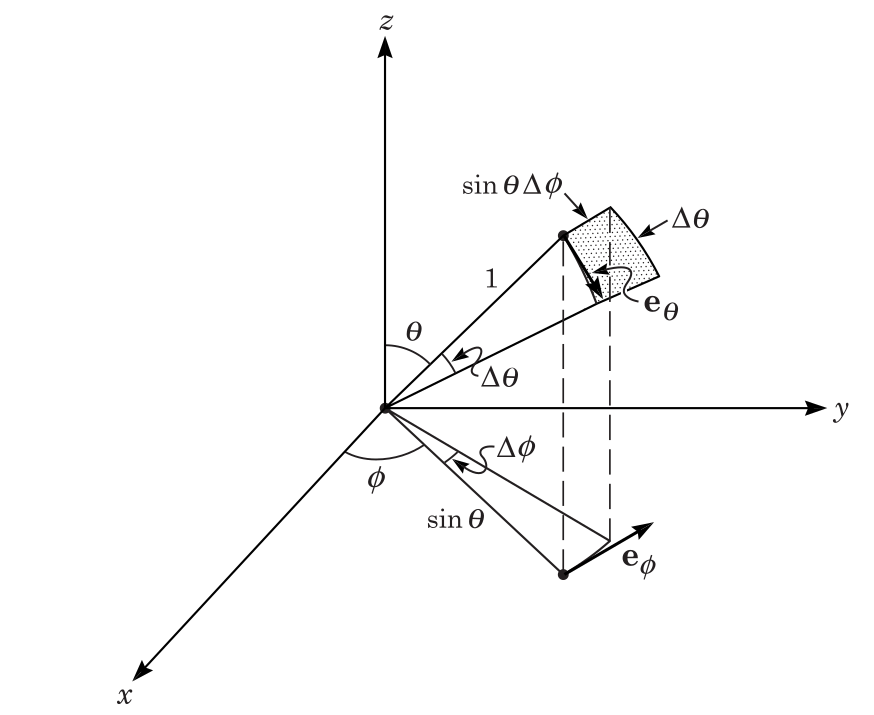
\includegraphics[width=12cm]{./figures/7.png}
	\caption{用于描述单位球面上的定向位移$\Delta \mathbf{u}$的球面极坐标系}
	\label{用于描述单位球面上的定向位移的球面极坐标系}
\end{figure}

为了进一步深入研究,有必要对类蠕虫链的跃迁概率$\Phi(\Delta \mathrm{u};\mathrm{r},\mathrm{u})$的形式进行明确说明。为此,图\ref{用于描述单位球面上的定向位移的球面极坐标系}所示的球面极坐标系是最方便的。在单位球面上增大极角$\theta$方向和指向角$\phi$方向上的正交单位矢量分别用$\mathrm{e}_\theta$和$\mathrm{e}_\phi$表示。对方程(\ref{类蠕虫链弯曲能表达式})进行离散后,单位球沿$\mathrm{e}_\theta$和$\mathrm{e}_\phi$的小位移$\Delta \mathrm{u}=(\Delta \theta ,\sin \theta \ \Delta \phi)$引起的弯曲能,即\\
\begin{equation}
\beta\Delta U_0 =\frac{\lambda}{2\Delta s}|\Delta \mathrm{u}|^2 =\frac{\lambda}{2\Delta s}[(\Delta\theta)^2+(\sin \theta \Delta \phi)^2]
\end{equation}
因此,跃迁概率$\Phi(\Delta \mathrm{u};\mathrm{r},\mathrm{u})\sim 
\exp(-\beta \Delta U_0)$是一个高斯分布,且有一阶矩和二阶矩\\
\begin{equation}
\langle \Delta \mathrm{u}\rangle_\Phi =0,\quad \langle \Delta \mathrm{u}\Delta \mathrm{u}\rangle_\Phi =\frac{\Delta s}{\lambda}(\mathrm{e}_\theta \mathrm{e}_\theta+\mathrm{e}_\phi \mathrm{e}_\phi)
\end{equation}
将此结果代入方程(\ref{Fokker-Planck方程})将得到所需的Fokker-Planck方程(Hermans和Ullman,1952)\\
\begin{equation}
	\frac{\partial}{\partial s}p_0(\mathrm{r},\mathrm{u},s) =-\mathrm{u} \cdot \nabla_\mathrm{r} \ p_0(\mathrm{r},\mathrm{u},s)+\frac{1}{2\lambda}\nabla_\mathrm{u}^2\  p_0(\mathrm{r},\mathrm{u},s)\label{简化的Fokker-Planck方程}
\end{equation}
其中$\nabla_\mathrm{u}^2$表示单位球面上的拉普拉斯算子\\
\begin{equation}
\nabla_\mathrm{u}^2 f \equiv \frac{1}{\sin\theta}\frac{\partial}{\partial\theta}\left(\sin\theta \frac{\partial f}{\partial \theta}\right)+\frac{1}{\sin^2\theta}\frac{\partial^2f}{\partial\phi^2}
\end{equation}
这个算子通常被称为\textbf{旋转扩散算子},因为它在单位球面上产生扩散运动(Berne和Pecora,1976)。在方程(\ref{简化的Fokker-Planck方程})中,参数$1/(2\lambda)$乘以$\nabla_\mathrm{u}^2$可以看作是一个\textbf{旋转扩散系数}。\\

Fokker-Planck 方程(\ref{简化的Fokker-Planck方程})提供了沿蠕虫状聚合物链的关于链段位置和指向传播的完整信息。这个方程显然没有一个简单的封闭形式的解析解,尽管它的空间傅里叶变换可以用连续分式展开(Spakowitz和Wang,2004)。关于数值方法的讨论将推迟到第3.6节。\\

如果我们将注意力限制在指向相关性上,那么很容易引入第二个约化分布函数\\
\begin{equation}
	H_0(\mathrm{u},s)\equiv\int d\mathrm{r}\ p_0(\mathrm{r},\mathrm{u},s)\label{第二个约化分布函数}
\end{equation}
它可以解释为一条轮廓长度$s$的蠕虫状链的末端具有指向$\mathrm{u}$的概率密度。将$H_0(\mathrm{u},s)$归一化,使得$\int d\mathrm{u}\  H_0(\mathrm{u},s)=1$。在周期边界条件下,可对方程(\ref{简化的Fokker-Planck方程})在$\mathrm{r}$上积分,得到约化指向分布函数的Fokker-Planck方程\\
\begin{equation}
	\frac{\partial}{\partial s}H_0(\mathrm{u},s)=\frac{1}{2\lambda}\nabla_\mathrm{u}^2\ H_0(\mathrm{u},s)\label{约化指向分布函数的Fokker-Planck方程}
\end{equation}
这个方程现在是一个简单的旋转扩散方程,它具有解析解(Berne和Pecora,1976;Saito等人,1967)。为此,很容易在$H_0(\mathrm{u},s)$上引入球谐函数展开,\\
\begin{equation}
	H_0(\mathrm{u},s)=\sum_{l=0}^{\infty}\sum_{m=-l}^{l}h_{lm}(s)Y_{lm}(\mathrm{u})\label{球谐函数展开}
\end{equation}
其中球谐函数$Y_{lm}(\mathrm{u})$是旋转扩散算子的特征函数
\begin{equation}
\nabla_\mathrm{u}^2Y_{lm}(\mathrm{u}) =-l(l+1)Y_{lm}(\mathrm{u})
\end{equation}

这些函数有不同的定义(Edmonds,1974)。在这里,我们采用了量子力学中常见的惯例(Schiff,1968),并对整数$l,m\geq 0$,定义$Y_{lm}(\mathrm{u})$\\
\begin{equation}
Y_{lm}(\mathrm{u}) = Y_{lm}(\theta,\phi)=(-1)^m\left[\frac{2l+1}{4\pi}\frac{(l-m)!}{(l+m)!}\right]^{1/2}P_l^m(\cos \theta )\ \exp(im\phi)
\end{equation}
其中$P_l^m(x)$与勒让德函数相关,定义为对整数$l,m\geq 0$,有\\
\begin{equation}
P_l^m(x)=(1-x^2)^{m/2}\frac{d^m}{dx^m}P_l(x)
\end{equation}
且$P_l(x)$是常见的勒让德多项式,\\
\begin{equation}
P_l(x)=\frac{1}{2^ll!}\frac{d^l}{dx^l}(x^2-1)^l\quad l\geq 0
\end{equation}
对负整数m的球谐函数用对称性定义\\
\begin{equation}
Y_{l,-m}(\theta,\phi) =(-1)^m Y_{lm}^*(\theta,\phi)
\end{equation}
星号表示复共轭。它们在某种意义上是正交的\\
\begin{equation}
\begin{aligned}
\int d\mathrm{u} \left[Y_{lm}(\mathrm{u})\right]^*Y_{l'm'}(\mathrm{u})&=\int_{0}^{2\pi}d\phi\int_{0}^{\pi}d\theta\sin\theta\left[Y_{lm}(\theta,\phi)\right]^*Y_{l'm'}(\theta,\phi)\\&=\delta_{ll'}\delta_{mm'}
\end{aligned}
\end{equation}
并为单位球面上的函数展开构建了一组完全基。\\

将方程(\ref{球谐函数展开})代入方程(\ref{约化指向分布函数的Fokker-Planck方程}),可写出旋转扩散方程的通解
\begin{equation}
H_0(\mathrm{u},s)=\int d\mathrm{u}'\ G(\mathrm{u},\mathrm{u}',s)H_0(\mathrm{u}',0)
\end{equation}
这个表达式的核心是具有以下球谐函数展开的格林函数:\\
\begin{equation}
G(\mathrm{u},\mathrm{u}',s) = \sum_{l=0}^{\infty}\sum_{m=-l}^{l}\left[Y_{lm}(\mathrm{u}')\right]^*Y_{lm}(\mathrm{u})\exp[-sl(l+1)/(2\lambda)]
\end{equation}
$G(\mathrm{u},\mathrm{u}',s)$描述了轮廓长度s的链段具有指向$\mathrm{u}$的末端和指向$\mathrm{u}'$的起始端的条件概率。这个格林函数对于分析理想类蠕虫链的统计性质特别有用。

一些主要感兴趣的是\textbf{指向相关函数orientational correlation function}\\
\begin{equation}
	\langle \mathrm{u}(s)\cdot \mathrm{u}(s')\rangle =\frac{1}{4\pi}\int d\mathrm{u}\int d\mathrm{u}'\mathrm{u}\cdot \mathrm{u}'G(\mathrm{u},\mathrm{u}',|s-s'|)\label{指向相关函数}
\end{equation}
对于计算这类相关函数,一个方便的公式是球谐函数加法定理(Edmonds,1974)\\
\begin{equation}
P_l(\mathrm{u}\cdot \mathrm{u}')=\frac{4\pi}{2l+1}\sum_{m=-l}^{l}[Y_{lm}(\mathrm{u})]^*Y_{lm}(\mathrm{u}')
\end{equation}
这个表达式的使用和方程(\ref{指向相关函数})中格林函数的球谐函数展开导致了\\
\begin{equation}
	\langle \mathrm{u}(s) \cdot \mathrm{u}(s')\rangle=\exp(-|s-s'|/\lambda)\label{简化的指向相关函数}
\end{equation}
微观长度λ的物理解释变得清楚;λ是\textbf{持续长度},即沿着蠕虫状链的轮廓定向相关衰减的距离。\\

上述结果可用于推导类蠕虫链端到端向量的均方。从表达\\
\begin{equation}
R^2 \equiv\langle|\mathrm{r}(L_c)-\mathrm{r}(0)|^2\rangle =\int_{0}^{L_c}ds \int_{0}^{L_c}ds'\langle \mathrm{u}(s)\cdot \mathrm{u}(s')\rangle
\end{equation}
插入(\ref{简化的指向相关函数}),我们得到\\
\begin{equation}
	R^2 =2\lambda\{L_c-\lambda[1-\exp(-L_c/\lambda)]\}\label{端到端向量的均方}
\end{equation}
这个表达式是在柔性理想链和刚性杆的性质之间连续插值的。在柔性极限中,它对应的轮廓长度远大于持久长度,$L_c/\lambda \gg 1$,方程(\ref{端到端向量的均方})化简为\\
\begin{equation}
R\approx(2\lambda L_c)^{1/2} \quad (L_c/\lambda \gg 1)
\end{equation}
这与自由连接链的理想链标度公式$R=bN^{1/2} 1$一致,如果我们选择将$N=L_c/\lambda$解释为统计独立的持久段数并令$b=\sqrt{2}\lambda$。相反的极限$L_c/\lambda \ll 1$,方程(\ref{端到端向量的均方})化简为\\
\begin{equation}
R \approx L_c \quad (L_c/\lambda \ll 1)
\end{equation}
这显然是刚性杆聚合物的精确结果。因此,通过改变蠕虫类链模型中的两个参数$\lambda$和$L_c$,可以描述具有广泛骨架柔性的理想聚合物的统计力学。\\

在讨论完类蠕虫链之前,应该注意到一些作者考虑了模型的变体,其中$\mathrm{u}(s)$是一个单位向量这一约束是局部放松的(Freed,1972;Harris和Hearst,1966)。在这些变体中,引入了拉格朗日乘子,使$\mathrm{u}(s)$以某种全局平均方式具有单位幅度。另一种看似更自然的方法(Tagami,1969;Saito和Namiki,1956;Yamakawa,1997)是用调和势$U(\mathrm{u})=(3/2)|\mathrm{u}|^2$代替约束$|\mathrm{u}(s)=1|$,并改变方程(\ref{简化的Fokker-Planck方程})右手边的旋转扩散算子,有\\
\begin{equation}
	\frac{\partial}{\partial s}p_0(\mathrm{r},\mathrm{u},s)=-\mathrm{u}\cdot \nabla_\mathrm{r} \ p_0(\mathrm{r},\mathrm{u},s)+\frac{1}{2\lambda}\nabla_\mathrm{u}\cdot [(\nabla_\mathrm{u}U+\nabla_\mathrm{u})\ p_0(\mathbf{r},\mathbf{u},s)]\\abel{改变扩散算子后的Fokker-Planck方程}
\end{equation}
在这个方程中,$\mathrm{u}$不再被限制在单位球面上,因此相空间$(\mathrm{r},\mathrm{u})$与严格类蠕虫链的五维空间相比,是六维空间。很容易证明方程(\ref{改变扩散算子后的Fokker-Planck方程})与稳态解$p_0(\mathrm{r},\mathrm{u},\infty)\sim \exp[−U(\mathrm{u})]=\exp[−(3/2)|\mathrm{u}|^2]$是一致的。因此,在稳态的情况下,$\langle |u|^2\rangle=1$。这个Fokker-Planck方程与描述带有惯性粒子的布朗运动的方程密切相关,并且有一个精确的,尽管复杂的封闭形式的解(Chan-drasekhar,1943)。由于当我们考虑外部势中链的更真实的情况(第三章的主题)时,这个优势就失去了,因此在高维相空间中工作所增加的计算负担使得模型不像真正的蠕虫链那么理想。\\

最后,值得注意的是,类蠕虫链模型已被很好地扩展去描述螺旋线形成的趋势(Yamakawa,1997)。这一扩展对于建立与蛋白质和其他生物分子有关的统计力学模型具有重要意义。这些生物分子能够在溶液中形成二级结构。\\
\endinput
